\chapter{Sprint de preparation}

\section{Introduction}
Ce chapitre presente l'analyse fonctionnelle de l'application web integree et du chatbot IA destines aux etudiants et administrateurs de Code 212. L'objectif est de fournir une plateforme complète et interactive pour la gestion des cours, l'emission de certificats et l'assistance en temps reel via un chatbot intelligent. Cette analyse detaillee etablira des directives pour le developpement d'une interface utilisateur intuitive, mettant en avant les besoins et preferences des utilisateurs, tout en integrant des outils automatises pour une experience pedagogique optimisee. Un système convivial et performant servira de catalyseur pour une meilleure engagement et une acquisition des connaissances plus efficace chez les etudiants.

\section{Methodologie Scrum et ses rôles}

Scrum est une methodologie agile utilisee principalement dans le developpement de logiciels pour gerer des projets complexes et assurer une livraison continue de produits de haute qualite. Elle repose sur des cycles de developpement iteratifs et incrementaux appeles "sprints", qui durent generalement de deux à quatre semaines. Scrum encourage la collaboration, la flexibilite et l'amelioration continue à travers des revues regulières et des retrospectives.

\subsection{Les rôles dans Scrum}

\begin{itemize}
    \item \textbf{Product Owner (PO)} \\
    L'equipe de developpement est composee de professionnels qui travaillent ensemble pour livrer des increments de produit potentiellement livrables à la fin de chaque sprint. L'equipe est auto-organisee et interdisciplinaire, possedant toutes les competences necessaires pour accomplir le travail sans dependre d'autres personnes exterieures à l'equipe.
\end{itemize}

\begin{figure}[H]
\centering
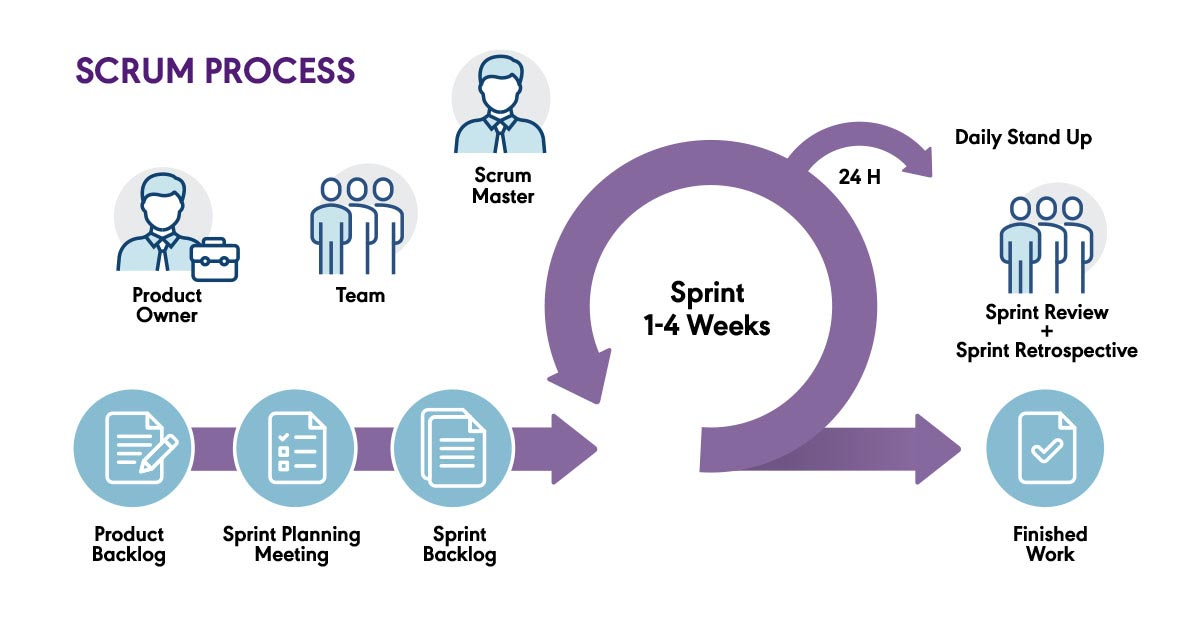
\includegraphics[width=\textwidth]{assets/images/scrum.jpg}
\caption{Methodologie Scrum}
\label{fig:methodologie_scrum}
\end{figure}

\section{Conclusion}
En conclusion, ce chapitre a mis en lumière la methodologie appliquee dans la conduite du projet de developpement du chatbot IA pour Code 212. L'approche methodique de la conception, la rigueur de la planification des tâches et l'agilite du developpement ont façonne un outil prometteur pour l'enrichissement de l'experience educative des etudiants. La maturite du processus adopte reflète notre engagement envers les valeurs d'excellence, de reactivite aux besoins des utilisateurs et d'innovation constante.

L'interaction entre la technologie de pointe et la pedagogie moderne de Code 212, incarnee par le chatbot IA, est destinee à etablir un nouveau standard en matière d'assistance etudiante en temps reel. Avec la fin de ce chapitre, nous anticipons la transition vers les phases subsequentes de mise en œuvre, d'evaluation et d'optimisation, qui seront abordees dans les chapitres suivants. L'impact positif attendu du chatbot sur l'accès à l'information et l'autonomie des etudiants suggère une transformation significative de leur parcours d'apprentissage numerique.

\section{Identification des Besoins Utilisateurs}
